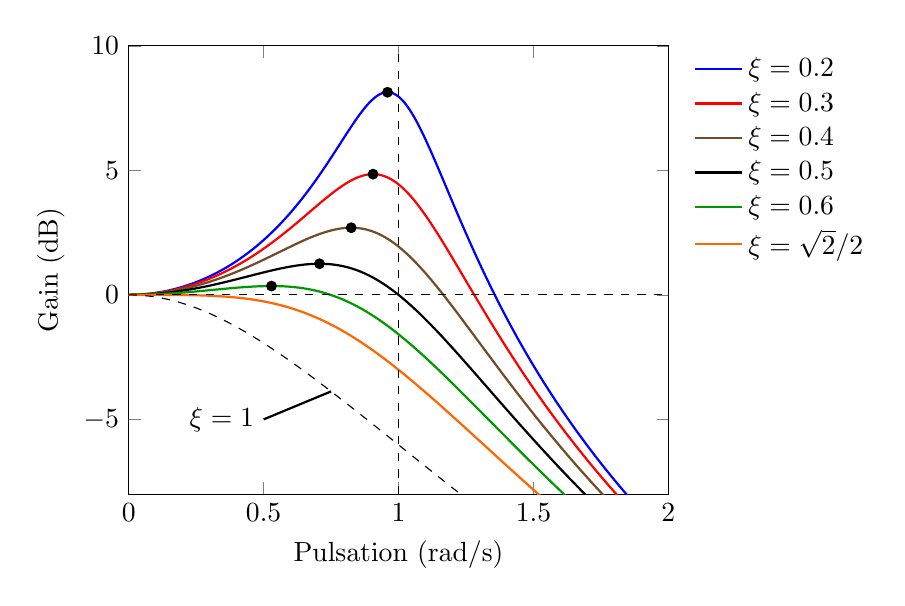
\begin{tikzpicture}
    \pgfplotscreateplotcyclelist{mycolorlist}{%
            blue\\%
            red\\%
            brown!60!black\\%
            black\\%
            green!60!black\\%
            red!60!yellow\\
            }
    \begin{axis}
    [   ticklabel style = {font=\normalsize},
        legend style={draw=none},
        legend pos=outer north east,
        legend cell align={left},
        ylabel={Gain (dB)},
        xlabel={Pulsation (rad/s)},
        xmode=normal,ymode=normal,
        xmin=0.0, xmax=2,
        ymin=-8, ymax=10,
        major grid style={black!40},
        cycle list name=mycolorlist,
    ]
    \foreach \a in {0.2,0.3,0.4,0.5,0.6,0.707} 
    \addplot+[thick,domain=0:2,samples=201] 
    {-20*log10(sqrt((1-x*x)^2 +(2*\a*x)^2))};

    \addplot[dashed,domain=0.1:5,samples=201] {0};
    \def\a{1.0}
    \addplot[dashed,domain=0:2,samples=201] 
    {-20*log10(sqrt((1-x*x)^2 +(2*\a*x)^2))};
    \coordinate (P) at 
    (axis cs:0.75,{-20*log10(sqrt((1-0.75*0.75)^2 +(2*\a*0.75)^2 ))});
    \node[left] (a) at (axis cs:0.5,-5) {$\xi=1$};
    \draw [thick] (a.east) -- (P);
    \addplot[mark size=1.75pt,black,fill=black,mark=*,only marks] 
    coordinates {
            (0.959166304663,8.13608784305)
            (0.905538513814,4.84656106912)
            (0.824621125124,2.69540739954)
            (0.707106781187,1.24938736608)
            (0.529150262213,0.354575339209)
    };
    \draw[dashed] (axis cs:1,-10) -- (axis cs:1,10);
    \legend{$\xi=0.2$,$\xi=0.3$,$\xi=0.4$,$\xi=0.5$,$\xi=0.6$,$\xi=\sqrt{2}/2$}
    \end{axis}
\end{tikzpicture}

